%%%%%%%%%%%%%%%%%%%%%%%%%%%%%%%%%%%%%%%%%%%%%%%%%%%%%%%%%%%%%%%%%%%%%%%%%%%%%%%%
%2345678901234567890123456789012345678901234567890123456789012345678901234567890
%        1         2         3         4         5         6         7         8

%\documentclass[letterpaper, 10 pt, conference]{ieeeconf}  % Comment this line out if you need a4paper

\documentclass[a4paper, 10pt, conference]{ieeeconf}      % Use this line for a4 paper

\IEEEoverridecommandlockouts                              % This command is only needed if 
                                                          % you want to use the \thanks command

\overrideIEEEmargins                                      % Needed to meet printer requirements.

% See the \addtolength command later in the file to balance the column lengths
% on the last page of the document

% The following packages can be found on http:\\www.ctan.org
\usepackage{graphics} % for pdf, bitmapped graphics files
\usepackage{graphicx}
%\usepackage{epsfig} % for postscript graphics files
%\usepackage{mathptmx} % assumes new font selection scheme installed
%\usepackage{times} % assumes new font selection scheme installed
\usepackage{amsmath} % assumes amsmath package installed
\usepackage{amssymb}  % assumes amsmath package installed
\usepackage{tabularx}
\usepackage[table,xcdraw]{xcolor}
\usepackage{multicol}


\title{\LARGE \bf
Design, Implementation, and Control of an Underwater Legged Robot for Low-Signature Underwater Exploration% for the MDS Robot
}


\author{Alberto Perez Nunez$^{1}$, Matko Orsag$^{2}$, and Daniel M. Lofaro$^{3}$% <-this % stops a space
\thanks{$^{1}$Alberto Perez is a student in the Electrical Engineering Department, George Mason University.
{\tt\small (E-mail: apereznu@gmu.edu}}%
%        {\tt\small (E-mail: cward13@gmu.edu}}%
\thanks{$^{2}$Matko Orsag is faculty with the Department of Control and Computer Engineering, University of Zagreb, Croatia.
	{\tt\small (matko.orsag@fer.hr}}%
\thanks{$^{3}$Daniel Lofaro is faculty with the Department of Electrical and Computer Engineering, George Mason University, Fairfax, VA, USA.
	{\tt\small (Tel : +1-202-378-8964; E-mail: dan@danLofaro.com}}%
%        {\tt\small (E-mail: don.sofge@nrl.navy.mil}}%
}

%\thanks{*This work was performed in part at the Naval Research Laboratory and was funded by the Office of Naval Research under grant number N0001416WX01272, Mobile Autonomous Navy Teams for Information Surveillance and Search (MANTISS).  In addition this work was supported by NRL-LASR, ONR-SFRP, and DASL@GMU}% <-this % stops a space
 

\begin{document}



\maketitle
\thispagestyle{empty}
\pagestyle{empty}


%%%%%%%%%%%%%%%%%%%%%%%%%%%%%%%%%%%%%%%%%%%%%%%%%%%%%%%%%%%%%%%%%%%%%%%%%%%%%%%%
\begin{abstract}
When operating a submerged vehicle near the sea floor one of the primary sensors that are used are the cameras.
These cameras become obstructed by silt and other debris when the ground is disturbed by the thrust from the submerged vehicles screws/thrusters.
In many cases these visual sensors become useless in these conditions.
This paper shows works towards creating a robot that can operate near the sea floor while keeping the area silt/debris free and viewable.
Specifically, this paper shows the design of a multi-legged robot with long thin legs to reduces disturbances and vortexes caused by the robot's motion underwater.
Within the design is the ability to land on its feet by being able to move its center of buoyancy during decent from the surface to the sea floor.
Control methods for achieving this are also included.
All design choices, FEA, load analysis, and other pertinent specification requirements are also included.
The result of this work is the design, fabrication, and creation of the IP-68 at 3 meters rated quadruped that has a tip to tip leg span of more than two meters.  
\end{abstract}


%%%%%%%%%%%%%%%%%%%%%%%%%%%%%%%%%%%%%%%%%%%%%%%%%%%%%%%%%%%%%%%%%%%%%%%%%%%%%%%%
\section{Introduction}
Submersibles operating near the oceans floor use cameras as one of their primary sensors.
This is especially true when operating when a low signature is required, i.e. not being able to use active sonar.
The submersible's cameras become obstructed by silt and other debris when the ground is disturbed by the thrust from the submerged vehicles screws/thrusters.
In may cases these visual sensors become useless in these conditions.
The overall goal of the overarching project is to create a system that can operate underwater in low signature environments while keeping visibility, mobility, and dexterity. 

This part of the project, and this paper, focuses on the initial design of a fully waterproof robot that can operate near/on the sea floor.
The robot is a multi-legged, where each leg is long and thin to reduce disturbances and vortexes caused by the robot's motion underwater.
In the future (but not in this paper) the legs will double as manipulators.
Within the design is the ability to land on its feet by being able to move its center of buoyancy.
This is so the robot can be deployed by dropping if off of the side of a surface vessel.
Control methods for achieving this behavior is included in this document.
All design choices, FEA, load analysis, and other pertinent specification requirements are also included.
All parts have been tested and simulated depths beyond the desired ratings.
The result of this work is the design, fabrication, and creation of the IP-68@3$m$ rated quadruped that has a tip to tip leg span of more than 2$m$.
The robot that was created can be seen in Figure~\ref{fig:cover}.
The final robot has been tested and fully functions underwater and can be see in Figure~\ref{fig:underwarter}.



\begin{figure}[!t]
\centering
\includegraphics[width=1.0\columnwidth]{img/aquashoko-2.pdf}
\includegraphics[width=1.0\columnwidth]{img/aquaShoko-fea-cad.pdf}
\caption{AquaShoko Robot: An IP-68 at 3$m$ rated underwater 12 degree of freedom quadruped designed for near/on sea floor for low signature underwater exploration.  The robot's long thin legs are designed to reduce disturbances and vortexes caused by the robot's motions. Future goals include adding manipulation abilities and autonomous operations. (Top Left) Real Robot, (Top Right) Simulated Robot in Gazebo Sim, (Bottom Left) CAD Model, and (Bottom Left) Finite Element Analyses of robot model. }
\label{fig:cover}
\end{figure}  



\section{Background}\label{sec:background}
The most recent underwater robot is the Ocean One by Khatib et. al. \cite{oceanone}.
The Ocean One is a high degree of freedom upper body humanoid robot with the lower body of an unmanned underwater vehicle (UUV).
This impressive robot can move around and manipulate objects with its highly sensitive tactile sensors on its manipulators.
The robot has been used to explore ship wrecks of historic interest and help excavate the artifacts.
The Ocean One is designed for its manipulation abilities.
The thrusters that allow the Ocean One to move through the water have the problem of most other UUVs where it stirs up silt and debris which reduces visibility.

\begin{figure*}[th]
\centering
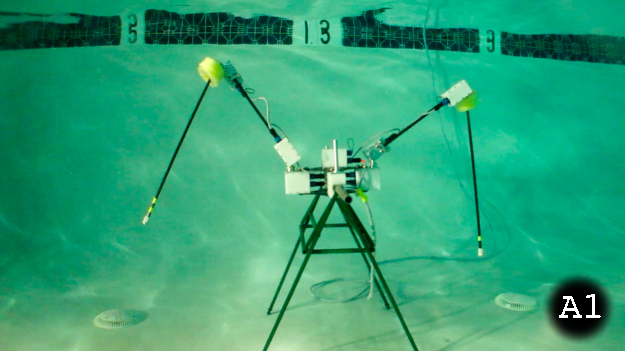
\includegraphics[width=0.66\columnwidth]{./img/a1.pdf}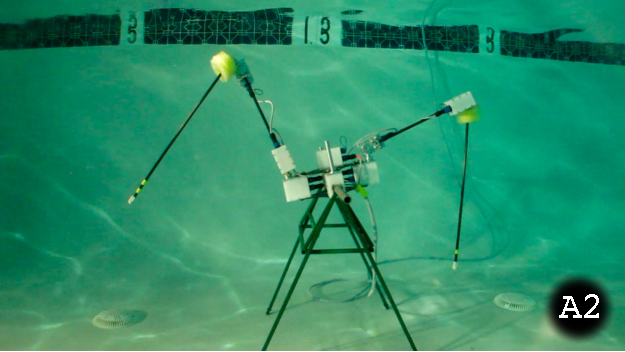
\includegraphics[width=0.66\columnwidth]{./img/a2.pdf}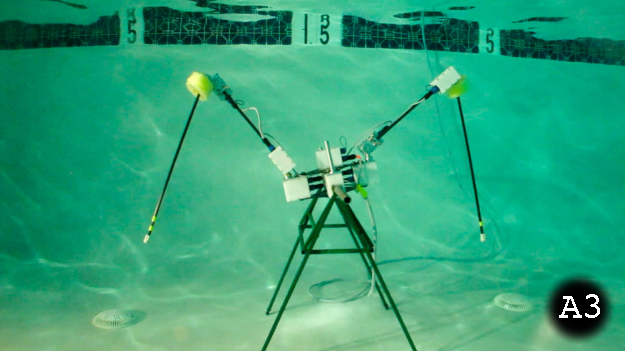
\includegraphics[width=0.66\columnwidth]{./img/a3.pdf}
\caption{AquaShoko underwater robot operating underwater controlling the attitude of its body via our method described in \ref{sec:stable}. The robot is being commanded with step input for the desired body attitude in the $Y-axis$ (out of the page).  (\textbf{A1-A3}) Step input of 0.2 $rad$, initial orientation 0.0 $rad$.  }
\label{fig:underwarter}
\end{figure*}


The Crabster (CR200) by the Korea Research Institute of Ships \& Ocean Engineering (KRISO) developed a legged underwater vehicle that does not need thrusters to move \cite{seacrab}.
It can navigate in upto 200$m$ water with passengers on board.
The legs of the robot were specifically designed to allow it to both swim and walk on the sea floor.
In their work they used the work of Kim et. al. \cite{crab1} and Jun et. al. for the communications and hydrodynamics of the legs respectively. 
These lessons help guide us in the choice of communication methods and size/shape of our legs.

Additionally JY Kim et. al. \cite{crab3} focused on creating a six-legged underwater UUV.
This is important because they also used their front two legs as manipulators.


From this previous work we decided to start by designing a legged robot with long thin legs to reduce the hydrodynamic effects.
Tethered communications and power was chosen for initial testing.
When adding manipulation in future work we will have six legs.  
Our current test platform has four legs because we want to focus on initial platform development before increasing the complexity of the system.



\section{Methodology}
\begin{figure}[h]
\centering
\includegraphics[width=1.0\columnwidth]{./img/aquaPod-evolution.png}
\caption{Waterproof actuator enclosure design iteration }
\label{fig:pod evolution}
\end{figure}


\subsection{IP68 Waterproof Enclosure}
An Aquapod is a waterproof enclosure design to house an MX-106 actuator to create a revolute joint. An Aquapod is to function as platform to build submersible robotic structures.
Requirements: 
\begin{itemize}
    \item Actuators cannot be modified 
    
    \item Ability for actuators to be daisy chained

    \item The bearing spun rough after test

    \item Waterproof to a minimum depth of 3 meters

    \item A compact package is required to maximize joint travel

    \item Fresh water corrosion resistant
    
\end{itemize}


\begin{figure}[h]
\centering
\includegraphics[width=1.0\columnwidth]{./img/aquaPod-exploded.png}
\caption{Exploited view of waterproof actuator enclosure }
\label{fig:pod exploted}
\end{figure}


This section describes the materials and components used for the Aquapod system.


\subsubsection{Actuators}
The MX-106T is a smart actuator which was chosen for its compact package and high torque capabilities. 
Specifications for MX-106T are listed below: 
\begin{itemize}
    \item Transistor-transistor Logic serial (TTl) communication 
    
    \item Recommended voltage: 12V

    \item No load speed at 12V: 45rpm

    \item Stall torque at 12V: 8.4 Nm

\end{itemize}

\subsubsection{Pod-Top}
Pod-Tops are intended to be the load bearing member. The actuator is bolted to the Pod-Top. The Pod-Top needs to house the shaft seal for the output shaft. The Pod-Top also needs to be able to transfer heat from the actuator to the environment. 
6061 Aluminum was chosen for its combination of low weight, high strength, high thermal conductivity, and machinability. To reduce production time, the Pod-Top geometry shape was developed to reduce waste stock.

\subsubsection{Output Shaft Seal}
Heavy duty, double-lip rotary seal is made to prevent water and other contaminates from entering the enclose. The rotary seal was working temperature range of 234K to 372K. The seal is rated for a pressure differential of 630kPa at 0 m/s and 344kPa at 5m/s. 


\subsubsection{Bearing Housing}
Bearing Housing secures the Output shaft bearing to the Pod-Top. Its job is to transfer the radial load from the bearing to the Pod-Top. The reason for using a separate bearing housing is to position the bearing as close to the load as possible to prevent the output shaft from pivoting and placing stress on the actuator.
6061 Aluminum was chosen for its combination of low weight, high strength, and machinability.

\subsubsection{Output Shaft Bearing}
Acetal bearing with stainless steel balls are used for their corrosion Resistance. Bearings have a static load rating of 244N and a dynamic load rating of 177N. 

\subsubsection{Pod-Bottom}
Pod-Bottoms mate with the Pod-Tops to create a water proof enclosure for the actuator. Pod-Bottoms protect the actuator from impacts. Pod-Bottoms are equipped with two panel mounted connectors to supply the actuator with power/ground and data connection. There are two version of Pod-Bottom one with link attachment points one without. The additional attachment points are used to increase structural rigidity. Pod-Bottoms are sealed with room temperature vulcanizing (RTV) silicone sealant and use a tight bolt pattern to ensure even pressure distribution between the Pod-Bottom and Pod-Top mating surfaces.
High Density Polyethylene was chosen for low weight, impact resistance and machinability. 

\subsubsection{IP68 Electrical Connectors}
Aquapods are design to use Bulgin 4000 series electrical connectors. 4000 series connectors are ideal due to their small size and ability to perform in harsh environments.  


\subsubsection{Output Shaft}
The output shaft transfers rotary motion from the actuator inside the Aquapod to the horn adapter outside the Aquapod.The output shaft transfers rotary motion from the actuator inside the Aquapod to the horn adapter outside the Aquapod.

\subsubsection{Horn adapter}
The Horn Adapter allows to connect the output shaft to links. The horn adaptor utilizes the original hole pattern of Dynamixels allowing for the possibility to interchange with OEM components.
Horn Adaptors are keyed into the Output Shaft and a bolt secures the horn against axial loading. 

\subsubsection{Fasteners}
Screws made from 18-8 stainless steel were chosen for their corrosion resistance. Socket head screws where chosen for ease of assembly in tight spaces and countered-bored holes.

\begin{figure}[h]
\centering
\includegraphics[width=1.0\columnwidth]{./img/aquaShoko-v3dot3-render-standPose.png}
\caption{Rendering of AquaShoko Version 3.3 standing pose}
\label{fig:shoko stand pose}
\end{figure}


\subsection{Submersible Quadruped}
AquaShoko is a quadruped built around the Aquapod platform which is submersible in fresh water. AquaShoko has the capability to traverse from a dry land environment to an underwater one. AquaShoko can orientate it itself by positioning its limbs to shift its center of buoyancy as it descends to the bottom of a pool. Each leg of has three degrees of freedom comprised of one yaw and two pitch joints. Currently each leg is identical and they’re place 90 degrees away from each other about the vertical center axis. 


This section describes the materials and components used for the quadruped named AquaShoko.


\begin{figure}[h]
\centering
\includegraphics[width=1.0\columnwidth]{./img/aquaShoko-v3dot3-exploded-assembly.png}
\caption{Exploded view of AquaShoko Components}
\label{fig:shoko exploded}
\end{figure}


\subsubsection{Frame}
AquaShoko uses two Frame members to connect the four legs together. The first frame secures the Pod-Tops together and a second one securing the Pod Bottoms together. At the center of each Frame are attachment holes to which components, such as sensor packs and batteries, can be secured to if needed. Carbon fiber laminate was chosen for its high stiffness and height weight.

\subsubsection{Horn-to-Horn}
The Horn-To-Horn allows for the two Aquapods in closely to create a joint with two perpendicular degrees of freedom.
6061 Aluminum was chosen for its combination of low weight, high strength, and machinability.

\subsubsection{Horn-to-Tube}
Horn-to-Tube allows the Horn Adaptor of the Aquapod to connect to a circular tube.
6061 Aluminum was chosen for its combination of low weight, high strength, and machinability.

\subsubsection{Pod-Top-to-Tube}
Pod-Top-to-Tube allows the Pod-Top of the Aquapod to connect to a circular tube.  
6061 Aluminum was chosen for its combination of low weight, high strength, and machinability.

\subsubsection{Femur and Tibia}
The Femur is a rod which connects the two pitch joints. The Tibia is the final link connected to the second pitch joint. Solid Nylon 6/6 rod in one inch on diameter was chosen for its high strength and low cost.

\subsubsection{Foot}
Slip-on rubber feet to prevent wear on the Tibia and improve traction for walking. 

\begin{figure}[h]
\centering
\includegraphics[width=1.0\columnwidth]{./img/aquaShoko-v3dot3-exploded-leg.png}
\caption{Exploded view of leg components:(a)Aquapod;(b)Horn-to-Horn;(c)Pod-Top-to-Tube;(d)Femur;(e)Horn-to-Tube;(f)Tibia;and (g)Foot}
\label{fig:leg exploded}
\end{figure}
 

\subsection{Power/Control Box}
The Power/Control Box is built around a Nema 4X rated enclosure to protect contents from possible slashing which occur around pools. The Power/Control Box is comprised of a Raspberry Pi2, DYN2USB adapter, power block, emergency button, key switch, Four cable outputs one cable input, a 12v to 5v power supply, and two 20 amp fuses. The power control box accepts a 12v input from a dell 120v AC to 12v power source.
The Raspberry can be connected to via local wifi network to operate. 
A DYN2USB adapter is used to connect the Raspberry Pi2 USB serial output to the TTL Dynamixel. 
The Power Block is used to distribute 12v power/ground to the cable outputs.
The emergency stop button is slash down resistant; it is used to cut power to all cable outputs in case of emergency.
The keyswitch switch is splash down resistant and is used to activate the dell power supply. The key switch prevents use of the robot by unauthorized persons. The 12v to 5v power source is used to power the Raspberry Pi2 and the TTL signal pull up resistor.
The two 20amp fuses protect the actuators.



\subsection{Power and Data Umbilical}
Three contact continuous flex cable rated for 10 amp was used to daisy chain connect the actuators and build the umbilical. IP68/IP69k rated water proof connectors were used.
The umbilical, which supplies power/grounds and data connection to AquaShoko, is approximately 12 meters long and uses two cables. The umbilical is wrapped in abrasion resistant sleeving to protect the cables if the umbilical is dragged across the ground. Due to the high 1.1ohm resistance of the umbilical and lower power of the Pi2 a pull up resistor was required to establish reliable connection. 

\begin{figure}[h]
\centering
\includegraphics[width=1.0\columnwidth]{./img/aquaShoko-v3dot2-photo-complete.JPG}
\caption{AquaShoko version 3.2 complete assembly }
\label{fig:shoko 3dot2}
\end{figure}

\subsection{Evaluating Maximum Joint Load Due To Gravity}
It is required for AquaShoko to be capable to walking on dry land for shore to near shore use. The maximum torque load due to gravity will occur when the leg is posed so the center of mass and the first pitch both lie on the same plane normal to the gravity vector. 

\begin{figure}[h]
\centering
\includegraphics[width=1.0\columnwidth]{./img/aquaShoko-v3dot3-legCOM.png}
\caption{Maximum joint load on leg due to gravity:(a)Second pitch joint;(b)Calculated center of mass;(c)First pitch joint;(d)Direction of gravity;(e)Reaction torque}
\label{fig:shoko 3dot2}
\end{figure}


\begin{align}\label{eq:head}
    T = FL   \\
    F = MG
\end{align}
\begin{align*}
    L & = 0.271 m         \\
    M & = 1.81 kg       \\
    G & = 9.81 m/s^2    \\
\end{align*}

The torque on the first pitch joint was calculated to be 4.81Nm which is 57.3\% of the of the actuators stall torque at 12V. This result is favorable because full range of motion is maintained when AquaShoko is not submerged.

\subsection{Finite Element Quadruped Structural Analysis}
Finite element stress and strain analysis was used to study the performance capabilities of the quadruped design structure. 
The following section will describe and discuss the results for structural studies done using Autodesk Fusion 360 simulation tool.

\subsubsection{Effector Point Load With Leg In Stand Pose }
It was desired to know how a leg posed in the standing position was subjected to a point load at the end effector. Using the stall torque of the actuator about the yaw joint a force of 24n was calculated and applied to the bottom of the the feet in the simulation. The Pod-Top of the yaw joint Aquapod was rigidly anchored. 
Interfering bodies where removed from the simulation such as electrical connectors and fasteners. All contacts where assumed to be bonded and contact tolerance was set to 0.5mm.


\subsection{Validating Finite Element Analysis Results}
Analytically engineering techniques where utilized to compare against the results of the finite element analysis. This was done to ensure the finite element result are within reasonable range of expected values.

\section{Testing}


\subsection{Aquapod water resistance testing}


\subsubsection{Shallow Submersion Test}
Test the water resistance of Aquapod in a shallow body of water.
Aquapod V3.1, without an actuator installed, was left in a 5 gallon bucket filled with tap water for a duration of 48 hours. 
No evidence of water ingress into the Aquapod nor electrical connectors; concluding a successful shallow submersion test.

Shallow Submersion Test observations:
\begin{itemize}
    \item Rust on the surface of black oxide steel hardware
    
    \item Rust on the surface of steel bearing

    \item The bearing spun rough after test

\end{itemize}

\begin{figure}[h]
\centering
\includegraphics[width=1.0\columnwidth]{img/rust.png}
\caption{(LEFT)Aquapod version 3.1 after first water resistance test, note the presence of rust.  (RIGHT)Aquapod version 3.1 moments after submersion, note the absence of rust.}
\label{fig:pod in bucket}\label{fig:pod rust}
\end{figure}





\subsubsection{Low Pressure Chamber Test}
Aquapods are expected to function reliably at a depth of 3m. A pressure chamber was used in order to simulate the proper depth. Using equation~\ref{eq:head}, the gauge pressure at 3m head to be 29.4kPa (4.2psi).

\begin{equation}\label{eq:head}
    P = \rho g h \\
\end{equation}

\noindent where P is gague pressure, $\rho$ is $1000 kg/m^3$, g is gravity, and h is the depth.

A factor of safety of 2.5 or higher is desired for water resistance. A minimum pressure benchmark for a successful test was calculated to be 73.6kPa (10.7psi), which simulates a depth of 7.5m.
The test took place over a 5 hour time span.
The pressure chamber was filled with tap water, and then the Aquapod V3.1, without an actuator installed, was submerged inside.
The source air pressure was initially adjusted to 241kPa (35psi) gauge and used initial pressurization of the chamber.
The source air was disconnected from the chamber and a gauge was used to measure the pressure inside the chamber to be 103kPa (15psi). 
The gauge was left connected for 5 minutes the pressure was observed to remained stable. 
The source air was then adjusted to 138kPa (20psi) gauge and left attached to the pressure chamber for the remainder of the test. 
Wet spots were observed, which indicated minor leakage occurred around the top of the pressure chamber; however, no evidence of moisture was found inside the Aquapod or any of the electrical connectors.
The test proved the Aquapod is water resistant beyond the 7.5m depth, which satisfies the desired factor of safety of 2.5.
This test also suggests Aquapods may be water resistant to or beyond 24m head; however, due to the air leakage, this claim cannot be confirmed and additional future testing is required.

Low pressure chamber test observations:
\begin{itemize}
    \item High pressure chamber is required for future tests
    
    \item Rust on the surface of steel bearing 
    
    \item More tests are required to determine the water resistance limit

    \item Design needs to be slightly modified for ease of dis-assembly

    \item Due to difficulty during dis-assembly, the mating surfaces of Pod-Bottom and Pod-Top were damaged
    
    \item An Aquapod must be tested in accord to IP68 standard procedures 
    
\end{itemize}

\begin{figure}[h]
\centering
\includegraphics[width=0.5\columnwidth]{./img/aquaPod-test-two-pressureCheck.JPG}\includegraphics[width=0.5\columnwidth]{./img/qr.jpg}
\caption{(RIGHT) Chamber internal gauge pressure during low pressure chamber test (LEFT) Video of AquaShoko being tested running the controller in \ref{sec:stable} under 1.5 $m$ of water.}
\label{fig:test two pressure check-1}\label{fig:video}
\end{figure}

\subsubsection{Physical Robot Underwater Test}
The physical robot was then tested for its ability to operate underwarter.  
Figure~\ref{fig:underwarter} shows the test of the robot running the body orientation algorithm defined in \ref{sec:stable}.
The depth of the robot is approximately 1.5 $m$.
The robot was tested for 1 hours continuously underwarter.
Figure~\ref{fig:video} is a link to the video for the AquaShoko test depicted in Figure~\ref{fig:underwarter} on the real robot under 1.5 $m$ of water.









%\section{Results}
%\input{Results.tex}

\section{Conclusion}
In conclusion we have created a multi-legged robot that is IP-68 rated at 3$m$ which is specifically designed for our overarching goal of creating a system that can operate underwater in low signature environments while keeping visibility, mobility, and dexterity.
This initial prototype has been tested using multiple types of mathematical analyses including FEA and physical testing including the use of a pressure chambers for simulated at depth conditions.
A dynamic simulation of the robot has been created in Gazebo and is controllable via its OpenSource controller called \textit{Shoko-Ach}.
Additionally the robot was designed to be able to move its center of buoyancy by moving its legs.
A controller has been designed for this robot to allow it to be thrown in the water at any angle and use its legs to ensure it lands on its feet.
Implementing the latter is immediate future work for this project.

\section*{Acknowledgements}
This work was performed by Lofaro Labs LLC and the DASL Group which includes the DASL Autonomous Systems Laboratory at the University of Zagreb (DASL@UNIZG) and the DASL Autonomous Systems Laboratory at George Mason University (DASL@GMU).




% references section
\bibliographystyle{IEEEtran}
\bibliography{aquashoko.bib,lofaro.bib,mds-ach.bib}


\end{document}
